%%%%%%%%%%%%%%%%%%%%%%%%%%%%%%%%%%%%%%%%%%%%%%%%%%%%%%
% A Beamer template for University of Wollongong     %
% Based on THU beamer theme                          %
% Author: Qiuyu Lu                                   %
% Date: July 2024                                    %
% LPPL Licensed.                                     %
%%%%%%%%%%%%%%%%%%%%%%%%%%%%%%%%%%%%%%%%%%%%%%%%%%%%%%
% Customized for Sharif University of Technology     %
%%%%%%%%%%%%%%%%%%%%%%%%%%%%%%%%%%%%%%%%%%%%%%%%%%%%%%


\documentclass[serif, aspectratio=169]{beamer}
%\documentclass[serif]{beamer}  % for 4:3 ratio
\usepackage[T1]{fontenc} 
\usepackage{fourier} % see "http://faq.ktug.org/wiki/uploads/MathFonts.pdf" for other options
\usepackage{hyperref}
\usepackage{latexsym,amsmath,xcolor,multicol,booktabs,calligra}
\usepackage{graphicx,pstricks,listings,stackengine}
\usepackage{lipsum}

\author{Ali Sharifi-Zarchi}
\title{Machine Learning (CE 40717)}
\subtitle{Fall 2024}
\institute{
    CE Department \\
    Sharif University of Technology
}
%\date{\small \today}
% \usepackage{UoWstyle}
\usepackage{SUTstyle}

% defs
\def\cmd#1{\texttt{\color{red}\footnotesize $\backslash$#1}}
\def\env#1{\texttt{\color{blue}\footnotesize #1}}
\definecolor{deepblue}{rgb}{0,0,0.5}
\definecolor{deepred}{RGB}{153,0,0}
\definecolor{deepgreen}{rgb}{0,0.5,0}
\definecolor{halfgray}{gray}{0.55}

\lstset{
    basicstyle=\ttfamily\small,
    keywordstyle=\bfseries\color{deepblue},
    emphstyle=\ttfamily\color{deepred},    % Custom highlighting style
    stringstyle=\color{deepgreen},
    numbers=left,
    numberstyle=\small\color{halfgray},
    rulesepcolor=\color{red!20!green!20!blue!20},
    frame=shadowbox,
}


\begin{document}

\begin{frame}
    \titlepage
    \vspace*{-0.6cm}
    \begin{figure}[htpb]
        \begin{center}
            
\includegraphics[keepaspectratio, scale=0.25]{pic/sharif-main-logo.png}
        \end{center}
    \end{figure}
\end{frame}

\begin{frame}    
\tableofcontents[sectionstyle=show,
subsectionstyle=show/shaded/hide,
subsubsectionstyle=show/shaded/hide]
\end{frame}

\section{Introduction}

\begin{frame}{Definition of Machine Learning (ML)}
\begin{itemize}
    \item \textbf{Machine Learning}: A field of study that enables computers to learn from data without being explicitly programmed.
    \item Involves constructing algorithms that generalize patterns from data.
    \item Focuses on predicting outcomes, classification, or uncovering hidden structures.
\end{itemize}
\end{frame}
\begin{frame}{Tom M. Mitchell's Definition of Machine Learning}
\begin{itemize}
    \item A well-known definition of machine learning comes from \textbf{Tom M. Mitchell}:
\end{itemize}
    \begin{quote}
    "A computer program is said to learn from experience E with respect to some class of tasks T and performance measure P, if its performance at tasks in T, as measured by P, improves with experience E."
    \end{quote}
\end{frame}

\begin{frame}{Definition of Machine Learning (cont.)}
\begin{itemize}
    \item \textbf{Goal}: Develop models that make accurate predictions based on past data.
    \item Formal definition: Given a task \(T\), performance measure \(P\), and experience \(E\):
    \[
    \text{Learning Problem} = (T, P, E)
    \]
    \item Example: Predicting house prices based on previous data.
\end{itemize}
\end{frame}

\begin{frame}{Example Usage of ML}
\begin{itemize}
    \item \textbf{Real-world examples}:
    \begin{itemize}
        \item Email Spam Detection (classification problem)
        \item Predicting House Prices (regression problem)
        \item Self-driving cars (real-time decision making)
    \end{itemize}
    \item Application domains: finance, healthcare, robotics, etc.
\end{itemize}
\end{frame}

\begin{frame}{Example Usage of ML: Home Price}
    \begin{minipage}{0.5\textwidth}
        \centering
        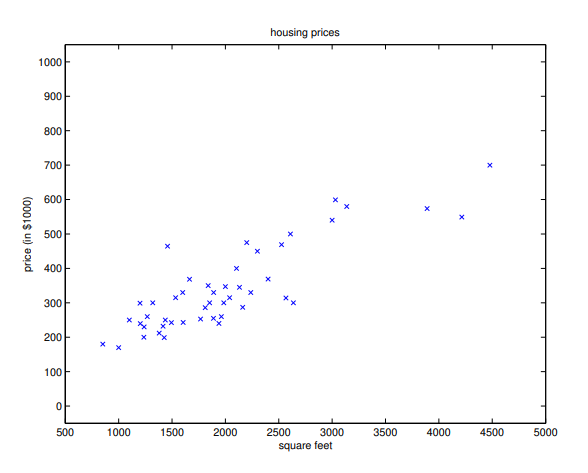
\includegraphics[width=0.9\textwidth]{pic/1.png}
        \captionof{Figure adopted from slides of Andrew Ng, Machine Learning course, Stanford.}
    \end{minipage}%
    \begin{minipage}{0.5\textwidth}
        \centering
        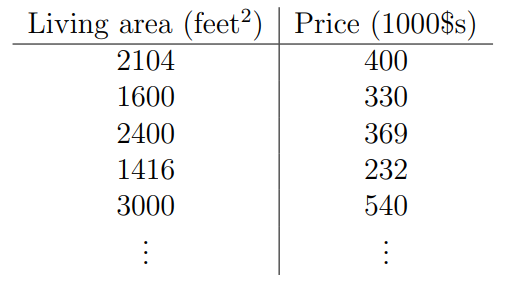
\includegraphics[width=0.9\textwidth]{pic/2.png}
    \end{minipage}
\end{frame}


\begin{frame}{Example Usage of ML: Applicant approval}
    \begin{minipage}{0.5\textwidth}
        \begin{itemize}
            \item Applicant form as the input.
            \item Output: approving or denying the request.
        \end{itemize}
    \end{minipage}%
    \begin{minipage}{0.5\textwidth}
        \centering
        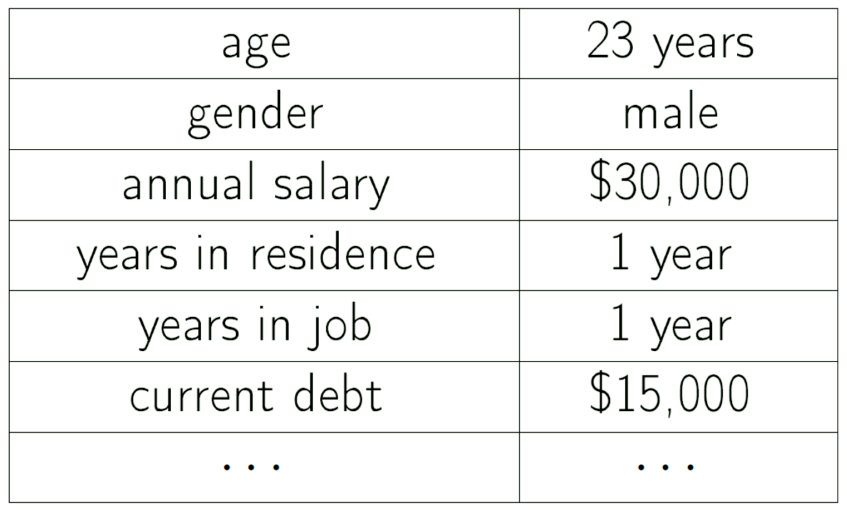
\includegraphics[width=0.9\textwidth]{pic/3.png}
        \captionof{Figure adopted from slides of Dr. Soleymani, Machine Learning course, Sharif University of technology.}
    \end{minipage}
\end{frame}

\begin{frame}{Paradigms of ML}

\begin{itemize}
    \item \textbf{Supervised learning} (regression, classification)
    \begin{itemize}
        \item predicting a target variable for which we get to see examples.
    \end{itemize}
    \item \textbf{Unsupervised learning}
    \begin{itemize}
        \item revealing structure in the observed data
    \end{itemize}
    \item \textbf{Reinforcement learning}
    \begin{itemize}
        \item partial (indirect) feedback, no explicit guidance
        \item Given rewards for a sequence of moves to learn a policy and utility functions
    \end{itemize}
    \item \textbf{Other paradigms:} semi-supervised learning, active learning, online learning, etc.
\end{itemize}

\end{frame}




\section{Supervised Learning }

\begin{frame}{Supervised Learning}
    \begin{itemize}
        \item \textbf{Definition}: A form of machine learning where the model learns from labeled data \( \{(x_i, y_i)\} \) to predict an output \( y \) given an input \( x \).
        \item \textbf{Goal}: Estimate a function \( f: \mathbb{R}^D \rightarrow \mathbb{R} \), such that \( y = f(x) + \epsilon \), where \( \epsilon \) is noise.
    \end{itemize}
\end{frame}

\begin{frame}
    \frametitle{Components of (Supervised) Learning}

    \begin{itemize}
        \item \textbf{Unknown target function:} \( f : \mathcal{X} \to \mathcal{Y} \)
        \begin{itemize}
            \item \textbf{Input space:} \( \mathcal{X} \)
            \item \textbf{Output space:} \( \mathcal{Y} \)
        \end{itemize}
        
        \vspace{0.5cm} % for spacing between points
        
        \item \textbf{Training data:} \( (x_1, y_1), (x_2, y_2), \ldots, (x_N, y_N) \)
        
        \vspace{0.5cm}
        
        \item \textbf{Pick a formula} \( g : \mathcal{X} \to \mathcal{Y} \) \textbf{that approximates the target function} \( f \)
        \begin{itemize}
            \item selected from a set of hypotheses \( \mathcal{H} \)
        \end{itemize}
    \end{itemize}
    
\end{frame}

\begin{frame}{Components of (Supervised) Learning (cont.)}
\begin{figure}[h]
  \centering
  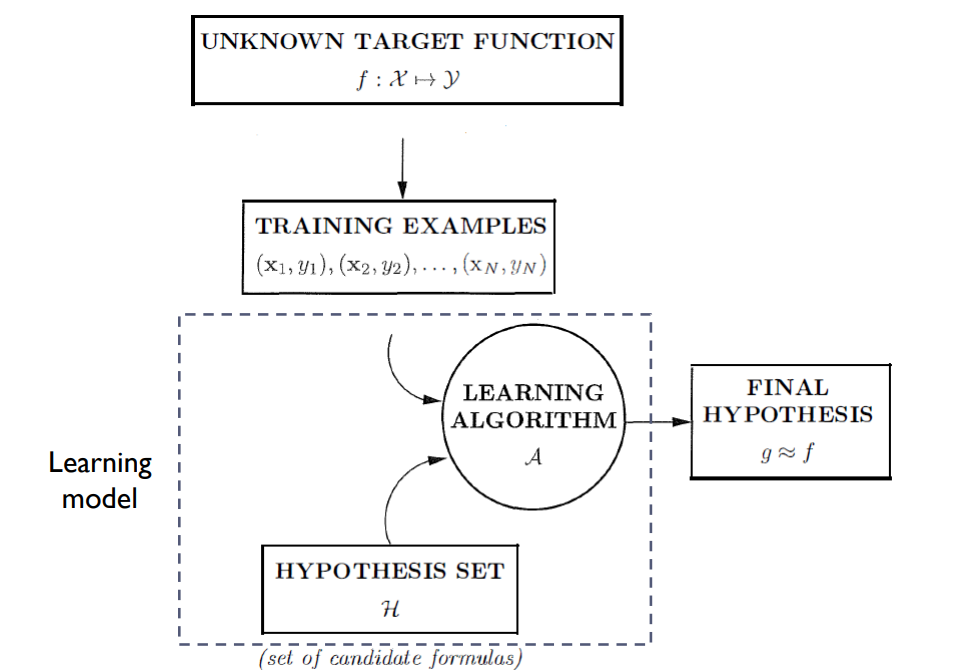
\includegraphics[width=0.7\linewidth]{pic/4.png}
\end{figure}
\end{frame}


\begin{frame}{Supervised Learning: Regression vs. Classification}

    \begin{itemize}
        \item \textbf{Regression}: predict a \underline{continuous} target variable
        \begin{itemize}
            \item E.g., $y \in [0, 1]$
        \end{itemize}
        \item \textbf{Classification}: predict a \underline{discrete} target variable
        \begin{itemize}
            \item E.g., $y \in \{1, 2, \ldots, C\}$
        \end{itemize}
    \end{itemize}

\end{frame}



\subsection{Linear regression}
\begin{frame}{Solution Components - Learning Model}
    \begin{itemize}
        \item The \textbf{Learning Model} consists of:
        \begin{itemize}
            \item \textbf{Hypothesis Set}: Defines the possible functions \( \mathcal{H} = \{h(x, \theta) | \theta \in \Theta\} \), where \( h(x, \theta) \) represents candidate functions.
            \item \textbf{Learning Algorithm}: Find \( \theta^* \in \Theta \) such that \( h(x, \theta^*) \approx f(x) \).
        \end{itemize}
        \item Both work together to map inputs \(x\) to outputs \(y\) with minimized error.
    \end{itemize}
    \vspace{0.5cm}
\end{frame}

\begin{frame}{Hypothesis Space Overview}
    \begin{itemize}
        \item \textbf{Hypothesis (h)}: A mapping from input space \( \mathcal{X} \) to output space \( \mathcal{Y} \).
        \item \textbf{Linear Regression Hypothesis}:
        \[
        h_{\mathbf{w}}(\mathbf{x}) = w_0 + w_1 x_1 + \dots + w_D x_D = \mathbf{w}^\top \mathbf{x}
        \]
        \item \textbf{Input Vector} \( \mathbf{x} \):
        \[
        \mathbf{x} = \begin{bmatrix} x_0 = 1, x_1, x_2, \dots, x_D \end{bmatrix}
        \]
        \item \textbf{Parameter Vector} \( \mathbf{w} \):
        \[
        \mathbf{w} = \begin{bmatrix} w_0, w_1, w_2, \dots, w_D \end{bmatrix}
        \]
    \end{itemize}
\end{frame}

\begin{frame}{Linear Hypothesis Representation}
    \begin{itemize}
        \item \textbf{Linear Hypothesis Space}:
        \begin{itemize}
            \item \textbf{Simplest form}: Linear combination of input features.
            \[
            h_{\mathbf{w}}(\mathbf{x}) = w_0 + \sum_{i=1}^{D} w_i x_i
            \]
        \end{itemize}
        \item \textbf{Linear Hypothesis Examples}:
        \begin{itemize}
            \item \textbf{Single Variable}: \( h_{\mathbf{w}}(x) = w_0 + w_1 x \)
            \item \textbf{Multivariate}: \( h_{\mathbf{w}}(\mathbf{x}) = w_0 + w_1 x_1 + w_2 x_2 \)
        \end{itemize}
    \end{itemize}
\end{frame}

\begin{frame}{Understanding Error Functions}
    \begin{itemize}
        \item In \textbf{hypothesis space}, we select a function \( h(x; \mathbf{w}) \) to approximate the true relationship between input \( x \) and output \( t \).
        \item The objective is to minimize the difference between predicted values \( h(x) \) and actual values \( t \).
        \item This difference is quantified using \textbf{error functions}, which guide us in choosing the optimal hypothesis.
    \end{itemize}
\end{frame}


\begin{frame}{What is an Error Function?}
    \begin{itemize}
        \item An \textbf{error function} measures how well the hypothesis \( h(x; \mathbf{w}) \) fits the training data.
        \item In regression problems, the most common error function is the \textbf{Sum of Squared Errors (SSE)}.
        \item Objective: Minimize the error function to find the best parameters \( \mathbf{w} \).
    \end{itemize}
    \[
    E(\mathbf{w}) = \sum_{n=1}^{N} \left( t_n - h(x_n; \mathbf{w}) \right)^2
    \]
\end{frame}

\begin{frame}{How to measure the error}

\begin{minipage}{0.5\textwidth}
    \centering
    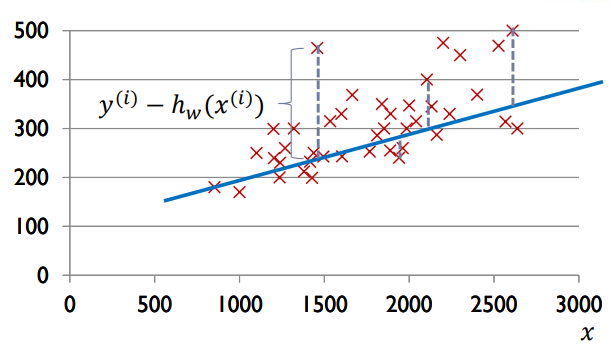
\includegraphics[width=\textwidth]{pic/6.png}
    \captionof{Figure adopted from slides of Dr. Soleymani, Machine Learning course, Sharif university of technology.}
\end{minipage}%
\begin{minipage}{0.5\textwidth}

    \[
    J(w) = \sum_{i=1}^{n} \left( y^{(i)} - h_w(x^{(i)}) \right)^2
    \]
    \[
    = \sum_{i=1}^{n} \left( y^{(i)} - w_0 - w_1 x^{(i)} \right)^2
    \]
\end{minipage}
\end{frame}

\begin{frame}{SSE: Sum of Squared Errors}
    \begin{itemize}
        \item \textbf{SSE} is widely used due to its simplicity and differentiability:
        \[
        SSE = \sum_{n=1}^{N} \left( t_n - \mathbf{w}^T \mathbf{x}_n \right)^2
        \]
        \item Intuitively, it represents the squared distance between predicted and true values.
        \item Penalizes larger errors more severely than smaller ones (due to the square).
    \end{itemize}
\end{frame}

\subsection{Analytical solution}
\begin{frame}{The learning algorithm}

\begin{itemize}
    \item \textbf{Choose} \( w \) \textbf{so as to minimize the} \( J(w) \)
    \[
    J(w) = \sum_{i=1}^{n} \left( y^{(i)} - h_w(x^{(i)}) \right)^2
    \]
    
    \item \textbf{The learning algorithm: optimization of the cost function}
    \begin{itemize}
        \item Explicitly taking the cost function derivative with respect to the \( w_i \)'s, and setting them to zero.
    \end{itemize}
    
    \item \textbf{Parameters of the best hypothesis for the training set:}
    \[
    w^* = \arg \min_{w} J(w)
    \]
\end{itemize}
\end{frame}


\begin{frame}{Cost function optimization: univariate}

\[
J(w) = \sum_{i=1}^{n} \left( y^{(i)} - w_0 - w_1 x^{(i)} \right)^2
\]

\begin{itemize}
    \item \textbf{Necessary conditions for the “optimal” parameter values:}
    \[
    \frac{\partial J(w)}{\partial w_0} = 0
    \]
    \[
    \frac{\partial J(w)}{\partial w_1} = 0
    \]
\end{itemize}

\end{frame}


\begin{frame}{Optimality conditions: univariate}

\[
J(w) = \sum_{i=1}^{n} \left( y^{(i)} - w_0 - w_1 x^{(i)} \right)^2
\]

\[
\frac{\partial J(w)}{\partial w_1} = \sum_{i=1}^{n} 2 \left( y^{(i)} - w_0 - w_1 x^{(i)} \right) (-x^{(i)}) = 0
\]

\[
\frac{\partial J(w)}{\partial w_0} = \sum_{i=1}^{n} 2 \left( y^{(i)} - w_0 - w_1 x^{(i)} \right) (-1) = 0
\]

\begin{itemize}
    \item A system of 2 linear equations
\end{itemize}

\end{frame}

\begin{frame}{Cost function optimization: multivariate}

\[
J(w) = \sum_{i=1}^{n} \left( y^{(i)} - h_w(x^{(i)}) \right)^2 = \sum_{i=1}^{n} \left( y^{(i)} - \mathbf{w}^T \mathbf{x}^{(i)} \right)^2
\]

\[
\mathbf{x} =
\begin{bmatrix}
1 & x_1^{(1)} & \cdots & x_d^{(1)} \\
1 & x_1^{(2)} & \cdots & x_d^{(2)} \\
\vdots & \vdots & \ddots & \vdots \\
1 & x_1^{(n)} & \cdots & x_d^{(n)}
\end{bmatrix}
\quad
\mathbf{w} =
\begin{bmatrix}
w_0 \\
w_1 \\
\vdots \\
w_d
\end{bmatrix}
\quad
\mathbf{y} =
\begin{bmatrix}
y^{(1)} \\
\vdots \\
y^{(n)}
\end{bmatrix}
\]

\end{frame}

\begin{frame}{Cost function optimization: multivariate}

\begin{itemize}
    \item \textbf{Explicitly taking the cost function derivative with respect to the} \( \mathbf{w} \)\textbf{, and setting them to zero.}
\end{itemize}

\[
J(\mathbf{w}) = \| \mathbf{y} - \mathbf{Xw} \|_2^2
\]

\[
\nabla_w J(\mathbf{w}) = -2 \mathbf{X}^T \left( \mathbf{y} - \mathbf{Xw} \right)
\]

\[
\nabla_w J(\mathbf{w}) = 0 \implies \mathbf{X}^T \mathbf{Xw} = \mathbf{X}^T \mathbf{y}
\]

\[
\mathbf{w} = \left( \mathbf{X}^T \mathbf{X} \right)^{-1} \mathbf{X}^T \mathbf{y}
\]

\begin{itemize}
    \item \textbf{Is} \( \mathbf{X}^T \mathbf{X} \) \textbf{invertible?}
\end{itemize}

\end{frame}


\begin{frame}{Cost function optimization}

\begin{itemize}
    \item \textbf{Another approach,}
    \begin{itemize}
        \item Start from an initial guess and iteratively change \( w \) to minimize \( J(w) \).
        \begin{itemize}
            \item The gradient descent algorithm
        \end{itemize}
    \end{itemize}
    
    \item \textbf{Steps:}
    \begin{itemize}
        \item Start from \( w^0 \)
        \item Repeat:
        \begin{itemize}
            \item Update \( w^t \) to \( w^{t+1} \) in order to reduce \( J \)
            \item \( t \leftarrow t + 1 \)
        \end{itemize}
        until we hopefully end up at a minimum.
    \end{itemize}
\end{itemize}

\end{frame}

\section{Optimization}

\subsection{Gradient descent}
\begin{frame}{Gradient Descent}

\begin{itemize}
    \item In each step, takes steps proportional to the negative of the gradient vector of the function at the current point \( w^t \):
    
    \[
    w^{t+1} = w^t - \eta \nabla J(w^t)
    \]
    
    \item \( J(w) \) \textbf{decreases fastest} if one goes from \( w^t \) in the direction of \( -\nabla J(w^t) \)
    
    \item \textbf{Assumption}: \( J(w) \) is defined and differentiable in a neighborhood of a point \( w^t \)
    
    \item \textbf{Gradient ascent} takes steps proportional to (the positive of) the gradient to find a local maximum of the function.
    
    \item Continue to find:
    
    \[
    w^* = \arg \min_w J(w)
    \]

\end{itemize}

\end{frame}

\begin{frame}{Gradient Descent (cont.)}

\begin{itemize}
    \item \textbf{Minimize} \( J(w) \)
\end{itemize}

\[
w^{t+1} = w^t - \eta \nabla_w J(w^t)
\]

\[
\nabla_w J(w) = 
\begin{bmatrix}
    \frac{\partial J(w)}{\partial w_1} \\
    \vdots \\
    \frac{\partial J(w)}{\partial w_d}
\end{bmatrix}
\]

\begin{itemize}
    \item If \( \eta \) is small enough, then \( J(w^{t+1}) \leq J(w^t) \).
    \item \( \eta \) can be allowed to change at every iteration as \( \eta_t \).
\end{itemize}

\end{frame}

\begin{frame}{Gradient descent disadvantages}

\begin{itemize}
    \item \textbf{Local minima problem}
    
    \item \textbf{However, when \( J \) is convex, all local minima are also global minima} \(\Rightarrow\) gradient descent can converge to the global solution.
\end{itemize}

\end{frame}

\begin{frame}{Problem of gradient descent with non-convex cost functions}

\begin{minipage}{0.5\textwidth}
    \centering
    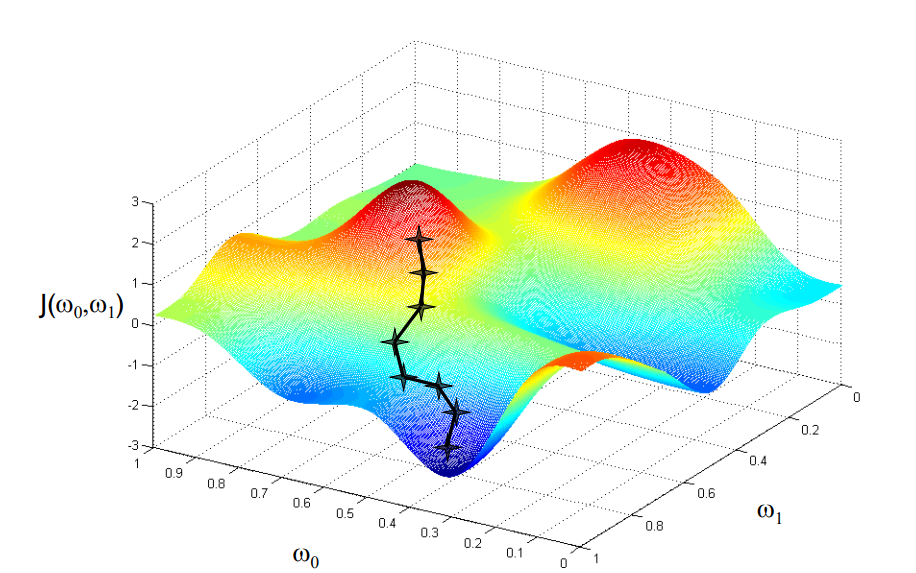
\includegraphics[width=\textwidth]{pic/7.png}
    \captionof{Figure adopted from slides of Andrew Ng, Machine Learning course, Stanford.}
\end{minipage}%
\begin{minipage}{0.5\textwidth}
    \centering
    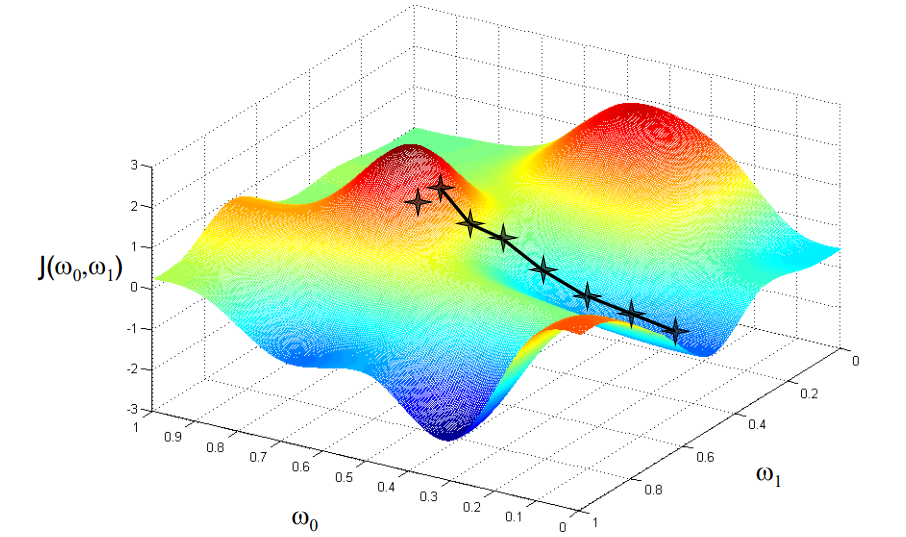
\includegraphics[width=\textwidth]{pic/8.png}
\end{minipage}

\end{frame}

\begin{frame}{Cost function optimization}

\begin{itemize}
    \item Weight update rule: $h_w(\mathbf{x}) = \mathbf{w}^T \mathbf{x}$
\end{itemize}

\[
\mathbf{w}^{t+1} = \mathbf{w}^t + \eta \sum_{i=1}^{n} \left( y^{(i)} - \mathbf{w}^T \mathbf{x}^{(i)} \right) \mathbf{x}^{(i)}
\]
\begin{center}
    \textit{Batch mode: each step considers all training data}
\end{center}

\begin{itemize}
    \item $\eta$: too small $\Rightarrow$ gradient descent can be slow.
    \item $\eta$: too large $\Rightarrow$ gradient descent can overshoot the minimum. It may fail to converge, or even diverge.
\end{itemize}

\end{frame}


\subsection{Stochastic gradient descent}
\begin{frame}{Stochastic gradient descent}

\begin{itemize}
    \item \textbf{Batch techniques} process the entire training set in one iteration
    \begin{itemize}
        \item Thus they can be computationally costly for large data sets.
    \end{itemize}
    \item \textbf{Stochastic gradient descent}: when the cost function can comprise a sum over data points:
\end{itemize}

\[
J(\mathbf{w}) = \sum_{i=1}^{n} J^{(i)}(\mathbf{w})
\]

\end{frame}

\begin{frame}{Stochastic gradient descent}

\begin{itemize}
    \item \textbf{Stochastic gradient descent}: when the cost function can comprise a sum over data points:
\end{itemize}

\[
J(\mathbf{w}) = \sum_{i=1}^{n} J^{(i)}(\mathbf{w})
\]

\begin{itemize}
    \item \textbf{Update after presentation of} $(\mathbf{x}^{(i)}, y^{(i)})$:
\end{itemize}

\[
\mathbf{w}^{t+1} = \mathbf{w}^t - \eta \nabla_{\mathbf{w}} J^{(i)}(\mathbf{w})
\]

\end{frame}

\begin{frame}{Stochastic gradient descent}

\begin{itemize}
    \item \textbf{Example:} Linear regression with SSE cost function
\end{itemize}

\[
J^{(i)}(\mathbf{w}) = \left( y^{(i)} - \mathbf{w}^T \mathbf{x}^{(i)} \right)^2
\]

\[
\mathbf{w}^{t+1} = \mathbf{w}^t - \eta \nabla_{\mathbf{w}} J^{(i)}(\mathbf{w})
\]

\[
\mathbf{w}^{t+1} = \mathbf{w}^t + \eta \left( y^{(i)} - \mathbf{w}^T \mathbf{x}^{(i)} \right) \mathbf{x}^{(i)}
\]

\end{frame}



\begin{frame}{Stochastic gradient descent: online learning}

\begin{itemize}
    \item \textbf{Sequential learning} is also appropriate for real-time applications
    \begin{itemize}
        \item Data observations are arriving in a continuous stream
        \item Predictions must be made before seeing all of the data
    \end{itemize}
\end{itemize}

\end{frame}

\begin{frame}{Stochastic gradient descent: online learning}

\begin{itemize}
    \item Often, stochastic gradient descent gets close to the minimum much faster than batch gradient descent.
    \item Note however that it may never converge to the minimum, and the parameters will keep oscillating around the minimum of the cost function;
    \begin{itemize}
        \item In practice, most of the values near the minimum will be reasonably good approximations to the true minimum.
    \end{itemize}
\end{itemize}

\end{frame}

\section{Probabilistic regression}
\begin{frame}{Introduction to Regression (Probabilistic Perspective)}
    \begin{itemize}
        \item Objective: Model the relationship between input \( \mathbf{x} \) and output \( y \).
        \item Uncertainty: Output \( y \) has an associated uncertainty modeled by a probability distribution.
        \item Example:
        \[
        y = f(\mathbf{x}; \mathbf{w}) + \epsilon, \quad \epsilon \sim \mathcal{N}(0, \sigma^2)
        \]
        \item The goal is to learn \( f(\mathbf{x}; \mathbf{w}) \) to predict \( y \).
    \end{itemize}
\end{frame}

\begin{frame}{Curve Fitting with Noise}
    \begin{itemize}
        \item In real-world scenarios, observed output \( y \) is noisy.
        \item Model: True output plus noise:
        \[
        y = f(\mathbf{x}; \mathbf{w}) + \epsilon, \quad \epsilon \sim \mathcal{N}(0, \sigma^2)
        \]
        \item Noise represents unknown or unmodeled factors.
        \item Example: Predicting house prices based on features with inherent unpredictability.
    \end{itemize}
\end{frame}

\begin{frame}{Expected Value of Output}
    \begin{itemize}
        \item Best Estimate: The conditional expectation of \( y \) given \( \mathbf{x} \).
        \[
        \mathbb{E}[y | \mathbf{x}] = f(\mathbf{x}; \mathbf{w})
        \]
        \item Goal: Learn a function \( f(\mathbf{x}; \mathbf{w}) \) that represents the average behavior of the data.
        \item Key Point: The model captures the mean of the target variable given input \( \mathbf{x} \).
    \end{itemize}
\end{frame}

\begin{frame}{Maximum Likelihood Estimation (MLE)}
    \begin{itemize}
        \item MLE: A method to estimate parameters that maximize the likelihood of the data.
        \item Given data \( \mathcal{D} = \{ (\mathbf{x}_i, y_i) \}_{i=1}^n \), MLE maximizes:
        \[
        L(\mathcal{D}; \mathbf{w}, \sigma^2) = \prod_{i=1}^n p(y_i | \mathbf{x}_i, \mathbf{w}, \sigma^2)
        \]
        \item Likelihood for regression:
        \[
        p(y | \mathbf{x}, \mathbf{w}, \sigma^2) = \frac{1}{\sqrt{2\pi \sigma^2}} \exp \left( - \frac{(y - f(\mathbf{x}; \mathbf{w}))^2}{2\sigma^2} \right)
        \]
        \item MLE finds: Parameters \( \mathbf{w} \) and \( \sigma^2 \) that best explain the data.
    \end{itemize}
\end{frame}

\begin{frame}{Univariate Linear Function Example}
    \begin{itemize}
        \item For a simple linear model \( f(\mathbf{x}; \mathbf{w}) = w_0 + w_1 x \):
        \[
        p(y | x, \mathbf{w}, \sigma^2) = \frac{1}{\sqrt{2\pi \sigma^2}} \exp \left( - \frac{(y - w_0 - w_1 x)^2}{2\sigma^2} \right)
        \]
        \item MLE Objective: Maximize the likelihood of the data points fitting the model.
        \item Key Observation: Points far from the fitted line will have a low likelihood value.
    \end{itemize}
\end{frame}

\begin{frame}{Log-Likelihood and Sum of Squares}
    \begin{itemize}
        \item Instead of maximizing the likelihood, it is often easier to maximize the log-likelihood:
        \[
        \log L(\mathcal{D}; \mathbf{w}, \sigma^2) = -n \log \sigma - \frac{n}{2} \log(2\pi) - \frac{1}{2\sigma^2} \sum_{i=1}^n (y_i - f(\mathbf{x}_i; \mathbf{w}))^2
        \]
        \item Equivalence: Maximizing the log-likelihood is equivalent to minimizing the Sum of Squared Errors (SSE):
        \[
        \sum_{i=1}^n (y_i - f(\mathbf{x}_i; \mathbf{w}))^2
        \]
    \end{itemize}
\end{frame}

\begin{frame}{Estimating \( \sigma^2 \)}
    \begin{itemize}
        \item The maximum likelihood estimate of the noise variance \( \sigma^2 \):
        \[
        \hat{\sigma}^2 = \frac{1}{n} \sum_{i=1}^n \left( y_i - f(\mathbf{x}_i; \hat{\mathbf{w}}) \right)^2
        \]
        \item Interpretation: Mean squared error of the predictions.
        \item Note: \( \sigma^2 \) reflects the noise level in the observations.
    \end{itemize}
\end{frame}

\begin{frame}{Maximum a Posteriori (MAP) Estimation}
    \begin{itemize}
        \item MAP: Incorporates prior information about parameters.
        \[
        \mathbf{w}_{MAP} = \arg \max_{\mathbf{w}} p(\mathbf{w} | \mathcal{D}) = \arg \max_{\mathbf{w}} p(\mathcal{D} | \mathbf{w}) p(\mathbf{w})
        \]
        \item Prior Distribution:
        \[
        p(\mathbf{w}) = \mathcal{N}(0, \alpha^2 I)
        \]
        \item Key Difference: Unlike MLE, MAP includes a prior to regularize the solution.
    \end{itemize}
\end{frame}

\begin{frame}{MAP as Regularized Least Squares}
    \begin{itemize}
        \item MAP estimation is equivalent to minimizing a regularized SSE:
        \[
        \mathbf{w}_{MAP} = \arg \min_{\mathbf{w}} \frac{1}{\sigma^2} \sum_{i=1}^n (y_i - f(\mathbf{x}_i; \mathbf{w}))^2 + \frac{1}{\alpha^2} \mathbf{w}^\top \mathbf{w}
        \]
        \item Regularization Term: \( \lambda = \frac{\sigma^2}{\alpha^2} \) controls how strongly the model is regularized.
    \end{itemize}
\end{frame}

\begin{frame}{Bayesian Approach}
    \begin{itemize}
        \item The Bayesian approach integrates over the distribution of parameters:
        \[
        p(y | \mathbf{x}, \mathcal{D}) = \int p(y | \mathbf{x}, \mathbf{w}) p(\mathbf{w} | \mathcal{D}) d\mathbf{w}
        \]
        \item This approach incorporates uncertainty in the parameters into the predictions.
        \item Benefit: Provides a probabilistic interpretation of the model’s predictions.
    \end{itemize}
    \textit{Reference: Slide 17}
\end{frame}

\begin{frame}{Predictive Distribution}
    \begin{itemize}
        \item In Bayesian linear regression, the predictive distribution is Gaussian:
        \[
        p(y | \mathbf{x}, \mathcal{D}) = \mathcal{N}(m_N^\top \mathbf{x}, \sigma_N^2(\mathbf{x}))
        \]
        \item \( m_N \): Posterior mean.
        \item \( \sigma_N^2(\mathbf{x}) \): Predictive variance.
        \item Key Point: This captures both the prediction and the uncertainty around it.
    \end{itemize}
    \textit{Reference: Slide 18}
\end{frame}

\begin{frame}{Prior and Posterior Distributions}
    \begin{itemize}
        \item Prior: Before seeing data, we assume a prior distribution on \( \mathbf{w} \):
        \[
        p(\mathbf{w}) = \mathcal{N}(0, \alpha^2 I)
        \]
        \item Posterior: After observing data, we compute the posterior distribution \( p(\mathbf{w} | \mathcal{D}) \).
        \item Bayesian Prediction: Integrates over the posterior to account for uncertainty.
    \end{itemize}
    \textit{Reference: Slide 18}
\end{frame}


\end{document}
